\documentclass[11pt,a4paper]{article}

\usepackage[a4paper,margin=1in]{geometry}
\usepackage{amsmath}
\usepackage{amssymb}
\usepackage{array}
\usepackage{booktabs}
\usepackage{enumitem}
\usepackage{tabularx}
\usepackage[T1]{fontenc}
\usepackage{lmodern}
\usepackage{tikz}
\usepackage{xcolor}

\definecolor{packblue}{RGB}{26,68,114}
\definecolor{packgrey}{RGB}{85,85,85}

\setlength{\parindent}{0pt}
\setlength{\parskip}{0.45em}
\setlist[enumerate,1]{label=(\alph*), leftmargin=1.1cm, itemsep=0.55em, topsep=0.4em}

\begin{document}

\begin{center}
{\Large\bfseries\color{packblue} Week 10 Revision Selected Questions}\\[0.4em]
{\large Worked Solutions}\\[0.3em]
{\color{packgrey} Based on \texttt{Sem 2 Week 10 - Revision.pdf}}
\end{center}

\vspace{0.8em}
\hrule
\vspace{1em}

\textbf{1. GreenGrid Energy}

Let $x_A,\ldots,x_F \in \{0,1\}$ where $x_i=1$ if project $i$ is selected.

\begin{enumerate}
\item A suitable binary model is
\[
\max Z = 14x_A+17x_B+11x_C+20x_D+9x_E+15x_F
\]
subject to
\[
6x_A+8x_B+5x_C+9x_D+4x_E+7x_F \le 21
\]
\[
x_D \le x_B
\]
\[
x_A+x_F \le 1
\]
\[
x_C+x_E \ge 1
\]
\[
x_i \in \{0,1\} \quad \text{for all projects } i.
\]

\item The optimal solution is
\[
x_B=x_D=x_E=1,\qquad x_A=x_C=x_F=0.
\]
Total cost:
\[
8+9+4=21
\]
Total benefit:
\[
17+20+9=46.
\]
So the best project set is $\{B,D,E\}$ with maximum total annual benefit score $46$.

\item Binary variables are required because each project is indivisible.
It is meaningful to choose or reject a project, but not to choose, for example, 0.4 of project $D$.

\item Add the constraint
\[
x_A+x_B+x_C+x_D+x_E+x_F=4.
\]
Under the budget and logic rules, there is no feasible solution selecting exactly four projects.
So the revised model is infeasible.

\item One realistic extension would be a multi-period capital budgeting model with separate yearly budgets and project timing decisions.
This would need extra data on when costs are incurred, when benefits begin, and any project sequencing dependencies.
\end{enumerate}

\newpage

\textbf{2. Hock-Brooke Automobiles}

Because the revision sheet does not specify a random-number stream or a simulation horizon, more than one valid simulation answer is possible.
Using the accompanying spreadsheet workbook, the intended approach is to show an illustrative short run and then estimate average cost from a much longer simulation.
The short table below is retained as an example, and the long-run recommendation is aligned to the spreadsheet results.

\begin{enumerate}
\item For capacity 9, one valid 12-week simulation is:

\begin{center}
\begin{tabular}{cccccccc}
\toprule
Week & Opening Stock & Delivered & Demand & Sales & Closing Stock & Overflow & Cost \\
\midrule
1 & 0 & 9 & 6 & 6 & 3 & 0 & 90 \\
2 & 3 & 8 & 7 & 7 & 4 & 0 & 90 \\
3 & 4 & 9 & 10 & 10 & 3 & 0 & 90 \\
4 & 3 & 10 & 7 & 7 & 6 & 0 & 90 \\
5 & 6 & 9 & 6 & 6 & 9 & 0 & 90 \\
6 & 9 & 8 & 8 & 8 & 9 & 0 & 90 \\
7 & 9 & 7 & 7 & 7 & 9 & 0 & 90 \\
8 & 9 & 9 & 8 & 8 & 10 & 1 & 110 \\
9 & 10 & 8 & 9 & 9 & 9 & 0 & 90 \\
10 & 9 & 10 & 6 & 6 & 13 & 4 & 170 \\
11 & 13 & 10 & 10 & 10 & 13 & 4 & 170 \\
12 & 13 & 9 & 7 & 7 & 15 & 6 & 210 \\
\bottomrule
\end{tabular}
\end{center}

This gives a short-run 12-week cost of
\[
1380
\]
and a short-run average weekly cost of
\[
\frac{1380}{12}=115.
\]

Using the spreadsheet logic over the long run, the estimated average weekly cost for capacity 9 is approximately
\[
103 \text{ per week}
\]
more precisely about 103.04 on the simulation sheet, and about 102.91 on the analysis sheet.

\item Using the spreadsheet analysis sheet, the estimated long-run average weekly costs are:

\begin{center}
\begin{tabular}{lc}
\toprule
Capacity & Average Weekly Cost \\
\midrule
6 & 110.74 \\
7 & 104.09 \\
8 & 102.16 \\
9 & 102.91 \\
10 & 106.89 \\
11 & 114.32 \\
\bottomrule
\end{tabular}
\end{center}

So, based on the spreadsheet outputs, capacity 9 is not the best choice.
The lowest long-run average cost is achieved at capacity 8, with an estimated average weekly cost of about 102.16.
Capacity 9 is only slightly worse, but the spreadsheet evidence supports recommending 8 spaces rather than 9.

Note: because no specific random-number stream was given in the source sheet, other correctly executed simulation runs may give slightly different short-run estimates.
\end{enumerate}

\newpage

\textbf{3. University Library Help Desk}

\begin{enumerate}
\item Main components:

Entities: students.

Resource: advisers.

Events: arrival, service start, service completion.

Stochastic inputs: interarrival times and service times.

Performance measures: number served, average wait, maximum wait and the percentage waiting less than 8 minutes.

\item One valid baseline run gives:

\begin{center}
\begin{tabular}{lc}
\toprule
Measure & Result \\
\midrule
Students served & 41 \\
Average wait & 1.17 minutes \\
Maximum wait & 10.32 minutes \\
\% waiting less than 8 minutes & 95.12\% \\
\bottomrule
\end{tabular}
\end{center}

\item Peak-period results:

\begin{center}
\begin{tabular}{lcccc}
\toprule
Advisers & Served & Avg wait & Max wait & \% below 8 min \\
\midrule
2 & 70 & 1.88 & 12.99 & 95.71\% \\
3 & 73 & 0.32 & 3.22 & 100.00\% \\
4 & 70 & 0.08 & 2.23 & 100.00\% \\
\bottomrule
\end{tabular}
\end{center}

The target is 97\% waiting less than 8 minutes.
The minimum staffing level that meets the target is therefore 3 advisers.

\item A \texttt{PriorityResource} can be used instead of an ordinary \texttt{Resource}.
Each arrival is labelled priority or standard, for example with probability 0.10 of being priority.
Priority users would request service with a smaller priority number, such as \texttt{priority=0}, while standard users might request with \texttt{priority=1}.
This would generally reduce waits for priority users and increase waits for standard users.

\item A single run is not enough because simulation output is affected by random variation.
Replications with different seeds give more stable estimates and allow the calculation of confidence intervals.
If the system were modelled as an ongoing operation rather than a fixed 360-minute session, a warm-up period could also be used to reduce start-up bias.
\end{enumerate}

\newpage

\textbf{4. F.B. Knight Deliveries}

Because the costs are stated per 10 items, it is convenient to model the variables in tens of items.
Then warehouse supplies are 10, 10 and 10, while shop demands are 7, 8 and 15.

\begin{enumerate}
\item Let
\[
x_{ij}=\text{number of tens of items shipped from warehouse }i\text{ to shop }j
\]
for
\[
i \in \{A,B,C\}, \qquad j \in \{X,Y,Z\}.
\]

The direct transportation network is:

\begin{center}
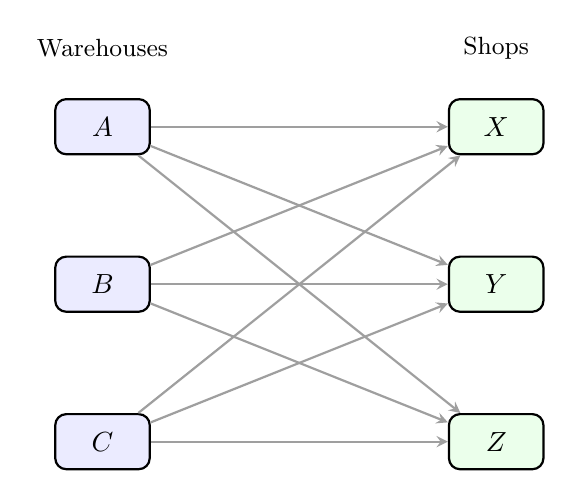
\begin{tikzpicture}[>=stealth, line width=0.8pt]
\node[draw, rounded corners, minimum width=1.2cm, minimum height=0.7cm, fill=blue!8] (A) at (0,2) {$A$};
\node[draw, rounded corners, minimum width=1.2cm, minimum height=0.7cm, fill=blue!8] (B) at (0,0) {$B$};
\node[draw, rounded corners, minimum width=1.2cm, minimum height=0.7cm, fill=blue!8] (C) at (0,-2) {$C$};
\node[draw, rounded corners, minimum width=1.2cm, minimum height=0.7cm, fill=green!8] (X) at (5,2) {$X$};
\node[draw, rounded corners, minimum width=1.2cm, minimum height=0.7cm, fill=green!8] (Y) at (5,0) {$Y$};
\node[draw, rounded corners, minimum width=1.2cm, minimum height=0.7cm, fill=green!8] (Z) at (5,-2) {$Z$};
\foreach \i in {A,B,C} {
  \foreach \j in {X,Y,Z} {
    \draw[->, gray!75] (\i) -- (\j);
  }
}
\node at (0,3) {\small Warehouses};
\node at (5,3) {\small Shops};
\end{tikzpicture}
\end{center}

The direct-shipping transportation model is
\[
\min Z =
8x_{AX}+7x_{AY}+5x_{AZ}
+12x_{BX}+3x_{BY}+9x_{BZ}
+10x_{CX}+11x_{CY}+7x_{CZ}
\]
subject to warehouse supply constraints
\[
x_{AX}+x_{AY}+x_{AZ}=10
\]
\[
x_{BX}+x_{BY}+x_{BZ}=10
\]
\[
x_{CX}+x_{CY}+x_{CZ}=10
\]
shop demand constraints
\[
x_{AX}+x_{BX}+x_{CX}=7
\]
\[
x_{AY}+x_{BY}+x_{CY}=8
\]
\[
x_{AZ}+x_{BZ}+x_{CZ}=15
\]
and non-negativity:
\[
x_{ij}\ge 0.
\]

One optimal direct-shipping plan is:

\begin{center}
\begin{tabular}{lcc}
\toprule
Route & Quantity (tens of items) & Cost per 10 items \\
\midrule
$A \to Z$ & 10 & 5 \\
$B \to X$ & 2 & 12 \\
$B \to Y$ & 8 & 3 \\
$C \to X$ & 5 & 10 \\
$C \to Z$ & 5 & 7 \\
\bottomrule
\end{tabular}
\end{center}

Total cost:
\[
10(5)+2(12)+8(3)+5(10)+5(7)=183.
\]

\item With the restrictions
\[
x_{BY}=0
\]
and
\[
x_{AY}\ge 0.5
\]
the same arc-variable model is modified by adding
\[
x_{BY}=0
\]
and
\[
x_{AY}\ge 0.5.
\]

In tens-of-items units, one optimal revised plan is:

\begin{center}
\begin{tabular}{lc}
\toprule
Route & Quantity (tens of items) \\
\midrule
$A \to Y$ & 8 \\
$A \to Z$ & 2 \\
$B \to X$ & 7 \\
$B \to Z$ & 3 \\
$C \to Z$ & 10 \\
\bottomrule
\end{tabular}
\end{center}

Revised total cost:
\[
8(7)+2(5)+7(12)+3(9)+10(7)=247.
\]
So the extra restrictions increase the cost from 183 to 247.

\item If direct shipping is not allowed and the intermediary locations are used, define arc variables
\[
y_{ik}=\text{flow from warehouse }i\text{ to intermediary }k
\]
for
\[
i \in \{A,B,C\}, \qquad k \in \{D_1,D_2\}
\]
and
\[
z_{kj}=\text{flow from intermediary }k\text{ to shop }j
\]
for
\[
k \in \{D_1,D_2\}, \qquad j \in \{X,Y,Z\}.
\]

The transhipment network is:

\begin{center}
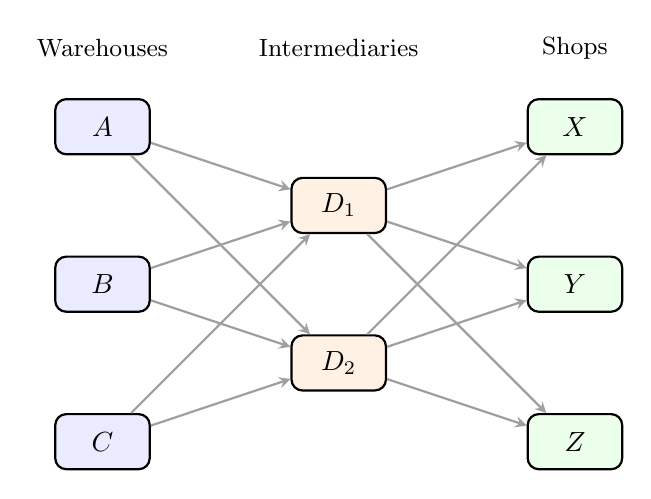
\begin{tikzpicture}[>=stealth, line width=0.8pt]
\node[draw, rounded corners, minimum width=1.2cm, minimum height=0.7cm, fill=blue!8] (A) at (0,2) {$A$};
\node[draw, rounded corners, minimum width=1.2cm, minimum height=0.7cm, fill=blue!8] (B) at (0,0) {$B$};
\node[draw, rounded corners, minimum width=1.2cm, minimum height=0.7cm, fill=blue!8] (C) at (0,-2) {$C$};
\node[draw, rounded corners, minimum width=1.2cm, minimum height=0.7cm, fill=orange!10] (D1) at (3,1) {$D_1$};
\node[draw, rounded corners, minimum width=1.2cm, minimum height=0.7cm, fill=orange!10] (D2) at (3,-1) {$D_2$};
\node[draw, rounded corners, minimum width=1.2cm, minimum height=0.7cm, fill=green!8] (X) at (6,2) {$X$};
\node[draw, rounded corners, minimum width=1.2cm, minimum height=0.7cm, fill=green!8] (Y) at (6,0) {$Y$};
\node[draw, rounded corners, minimum width=1.2cm, minimum height=0.7cm, fill=green!8] (Z) at (6,-2) {$Z$};
\foreach \i in {A,B,C} {
  \foreach \k in {D1,D2} {
    \draw[->, gray!75] (\i) -- (\k);
  }
}
\foreach \k in {D1,D2} {
  \foreach \j in {X,Y,Z} {
    \draw[->, gray!75] (\k) -- (\j);
  }
}
\node at (0,3) {\small Warehouses};
\node at (3,3) {\small Intermediaries};
\node at (6,3) {\small Shops};
\end{tikzpicture}
\end{center}

The transhipment model is
\[
\min Z =
4y_{AD_1}+5y_{AD_2}
+3y_{BD_1}+2y_{BD_2}
+6y_{CD_1}+4y_{CD_2}
+4z_{D_1X}+5z_{D_1Y}+2z_{D_1Z}
+2z_{D_2X}+4z_{D_2Y}+4z_{D_2Z}
\]
subject to supply constraints at the warehouses
\[
y_{AD_1}+y_{AD_2}=10
\]
\[
y_{BD_1}+y_{BD_2}=10
\]
\[
y_{CD_1}+y_{CD_2}=10
\]
demand constraints at the shops
\[
z_{D_1X}+z_{D_2X}=7
\]
\[
z_{D_1Y}+z_{D_2Y}=8
\]
\[
z_{D_1Z}+z_{D_2Z}=15
\]
and flow-balance constraints at the intermediary nodes
\[
y_{AD_1}+y_{BD_1}+y_{CD_1}=z_{D_1X}+z_{D_1Y}+z_{D_1Z}
\]
\[
y_{AD_2}+y_{BD_2}+y_{CD_2}=z_{D_2X}+z_{D_2Y}+z_{D_2Z}.
\]

All arc flows satisfy
\[
y_{ik}\ge 0, \qquad z_{kj}\ge 0.
\]

If only one intermediary is used, then the variables on the unused node are omitted from the model.
The three possibilities are:

\begin{center}
\begin{tabular}{lc}
\toprule
Intermediary choice & Total cost \\
\midrule
$D_1$ only & 228 \\
$D_2$ only & 216 \\
Both $D_1$ and $D_2$ & 181 \\
\bottomrule
\end{tabular}
\end{center}

So both intermediary locations should be used.

One optimal transhipment plan is:

\begin{center}
\begin{tabular}{lc}
\toprule
Route & Quantity (tens of items) \\
\midrule
$A \to D_1$ & 10 \\
$B \to D_1$ & 5 \\
$B \to D_2$ & 5 \\
$C \to D_2$ & 10 \\
$D_1 \to Z$ & 15 \\
$D_2 \to X$ & 7 \\
$D_2 \to Y$ & 8 \\
\bottomrule
\end{tabular}
\end{center}

Total cost:
\[
10(4)+5(3)+5(2)+10(4)+15(2)+7(2)+8(4)=181.
\]
This is slightly cheaper than the best direct-shipping plan.
\end{enumerate}

\newpage

\textbf{5. Forecasting at N\&F}

\begin{enumerate}
\item The quarterly data show a clear upward trend over time.
Using centred 4-quarter moving averages, the smoothed values where available are:

\begin{center}
\begin{tabular}{cc}
\toprule
Period & Centred 4-quarter moving average \\
\midrule
3 & 1020.250 \\
4 & 1030.500 \\
5 & 1040.750 \\
6 & 1050.625 \\
7 & 1060.500 \\
8 & 1070.375 \\
9 & 1080.375 \\
10 & 1090.625 \\
11 & 1100.875 \\
12 & 1111.125 \\
13 & 1121.250 \\
14 & 1131.000 \\
\bottomrule
\end{tabular}
\end{center}

\item Estimated seasonal variations:

Additive seasonal values:
\[
\text{Spring}=12.48,\quad
\text{Summer}=15.85,\quad
\text{Autumn}=-18.27,\quad
\text{Winter}=-10.06.
\]

Multiplicative seasonal indices:
\[
\text{Spring}=1.0117,\quad
\text{Summer}=1.0147,\quad
\text{Autumn}=0.9829,\quad
\text{Winter}=0.9907.
\]

\item A linear trend fitted to the centred moving averages is approximately
\[
\hat{T}_t = 990.12 + 10.07t.
\]

Forecasts for next year are therefore:

\begin{center}
\begin{tabular}{lccc}
\toprule
Period & Season & Additive Forecast & Multiplicative Forecast \\
\midrule
17 & Spring & 1173.74 & 1174.83 \\
18 & Summer & 1187.18 & 1188.53 \\
19 & Autumn & 1163.12 & 1161.18 \\
20 & Winter & 1181.40 & 1180.42 \\
\bottomrule
\end{tabular}
\end{center}

\item Both models give very similar forecasts.
However, the additive model is slightly easier to justify because the seasonal effects appear roughly constant in size over time, rather than increasing proportionally with the level of the series.
So an additive model would be a reasonable recommendation here, although either model would give very similar practical forecasts.
\end{enumerate}

\vfill

\begin{center}
\textit{End of Solutions}
\end{center}

\end{document}
